\section{Results}\label{sec:results}
The results are reported by research question, in the order set out in Section~\ref{sec:design}: RQ1 in Section~\ref{sec:res-rq1}, RQ2 in Section~\ref{sec:res-adaptation}, RQ3 in Section~\ref{sec:res-rq3} and RQ4 in Section~\ref{sec:res-rq4}. Each subsection is titled by its question and reports the primary analysis before the sensitivity analyses.

In summary, frozen COLIPRI had the highest discrimination on LUNG1 and exceeded \model{Stage+Volume} and radiomics in point estimate, by about 0.03 with 16 components and 0.045 with 32, but none of these differences was statistically significant after Holm correction, and no encoder significantly added to the clinical covariates (RQ1). Neither trainable heads nor encoder adaptation improved on the frozen linear head, and the encoders showed no advantage in label efficiency (RQ2). Only COLIPRI was sensitive to the tumour, and hiding the tumour inside any encoder lowered discrimination by at most 0.013 (RQ3). Externally, risk ordering by the stronger encoders transported, whereas their incremental clinical value remained unresolved and their absolute risks were miscalibrated (RQ4).

All internal estimates are mean-fold Uno C at 36 months on the 416 LUNG1 patients. Intervals are 95\% paired bootstrap intervals conditional on the fitted models, $p$ values are Holm-adjusted within the families of Section~\ref{sec:stats}, and ``equivalent'' means that the 90\% interval of a difference lay within the $\pm0.03$ margin.

\subsection{RQ1: How much prognostic information is accessible from frozen foundation-model representations, relative to clinical, radiomic and tumour-centred models?}\label{sec:res-rq1}

Frozen discrimination was modest for every model (Figure~\ref{fig:rq1}a). COLIPRI was the highest, at 0.617 (0.582 to 0.652), followed by TANGERINE (0.599), DINOv3 (0.575), Rad-JEPA-3D (0.539) and CT-CLIP (0.530). The clinical covariates alone were close to chance (\model{Clinical}, 0.529; 0.493 to 0.565), and \model{Stage+Volume} reached 0.588. The tumour-centred comparators ranged from 0.555 (Pai lesion encoder) to 0.591 (GTV radiomics). With the 32-component head (PCA32), a sensitivity analysis of head capacity added after the PCA16 comparisons (open markers in Figure~\ref{fig:rq1}a), COLIPRI reached 0.634 (0.600 to 0.669), followed by TANGERINE (0.607), DINOv3 (0.560), Rad-JEPA-3D (0.559) and CT-CLIP (0.527). Each encoder changed by $-0.014$ to $+0.020$ relative to PCA16, none significantly (Table~\ref{tab:trainable_results}), and the two leading encoders were the same with both heads.
\begin{figure}[!t]
\centering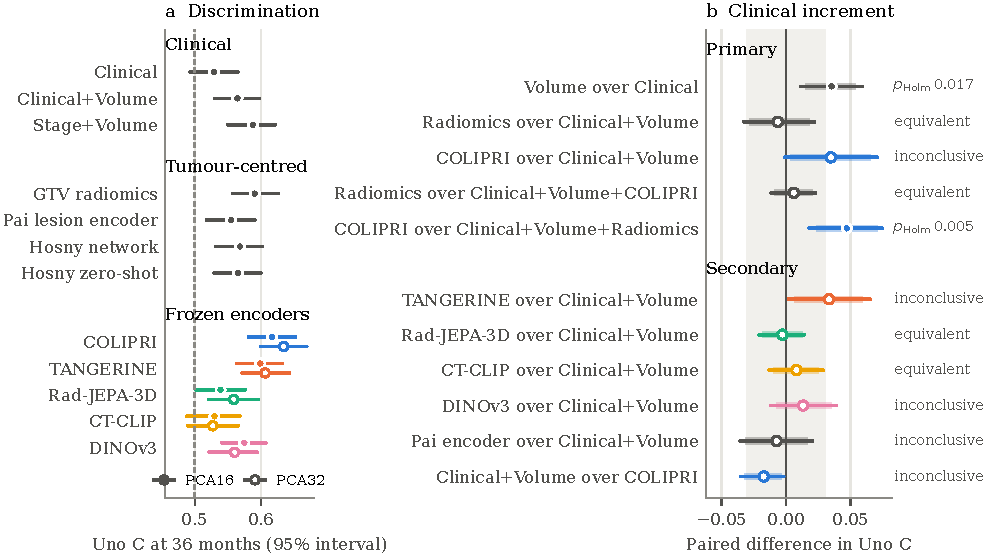
\includegraphics[width=\linewidth]{figures/results_rq1.pdf}
\caption{RQ1: frozen discrimination on LUNG1. (a) Uno C at 36 months with 95\% intervals for the clinical models, the tumour-centred comparators and the frozen encoders with the primary PCA16 linear Cox head (filled markers) and the PCA32 sensitivity head (open markers); the dashed line marks chance. (b) Paired differences between nested clinical models: thin lines, 95\% intervals; thick bands, 90\% intervals; shaded area, the $\pm0.03$ equivalence margin; filled markers, $p_\mathrm{Holm}<0.05$. The verdict on the right is ``equivalent'' when the 90\% interval lies within the margin and ``inconclusive'' when neither a difference nor equivalence was shown.}
\label{fig:rq1}
\end{figure}

No encoder differed from \model{Stage+Volume} or from GTV radiomics after Holm correction. COLIPRI exceeded them by 0.029 ($-0.015$ to 0.071) and 0.026 ($-0.015$ to 0.072), both with $p_\mathrm{Holm}=1.00$; the minimum detectable difference was about 0.06. The largest deficit was CT-CLIP against radiomics, $-0.061$ ($-0.114$ to $-0.009$; $p_\mathrm{Holm}=0.14$). With the 32-component head, a sensitivity analysis, COLIPRI reached 0.634 and exceeded \model{Stage+Volume} by 0.046 ($-0.001$ to 0.093) and radiomics by 0.043 (0.001 to 0.084); neither difference remained significant after Holm correction ($p_\mathrm{Holm}=0.38$ for both), and no other encoder exceeded either baseline. COLIPRI also exceeded the tumour-centred deep models, by 0.062 over the Pai lesion encoder ($p=0.009$, $p_\mathrm{Holm}=0.056$) and by 0.051 over Hosny zero-shot ($p_\mathrm{Holm}=0.14$), without reaching significance after correction.

The contrasts between nested clinical models fall into a primary and a secondary group (Figure~\ref{fig:rq1}b), which differ in the question they address rather than in the encoder. The primary contrasts follow the prespecified sequence of nested models, in which each step adds one block (tumour volume, radiomics, COLIPRI) to the previous model, and answer the main question of which information adds to the clinical covariates. The secondary contrasts lie outside this sequence and check its conclusions: they add each of the other four foundation models or the tumour-centred Pai lesion encoder to \model{Clinical+Volume}, and, in the reverse direction, add the clinical covariates and tumour volume to an image representation alone. The primary contrasts formed one Holm family and each type of secondary contrast its own, so that the supporting comparisons did not dilute the primary ones. In the primary family, tumour volume was the only block that added discrimination to the clinical covariates after correction: \model{Clinical+Volume} exceeded \model{Clinical} by 0.035 (0.011 to 0.059; $p_\mathrm{Holm}=0.017$). Radiomics added nothing to \model{Clinical+Volume} ($-0.006$; 90\% interval $-0.028$ to 0.018, equivalent). COLIPRI added 0.035 ($-0.001$ to 0.070; $p_\mathrm{Holm}=0.18$), a difference smaller than the minimum detectable difference of 0.052, so this contrast is inconclusive rather than negative. Once COLIPRI was in the model, radiomics again added nothing (0.006; 90\% interval $-0.009$ to 0.020, equivalent). Conversely, COLIPRI added to radiomics: \model{Clinical+Volume+Radiomics+COLIPRI} exceeded \model{Clinical+Volume+Radiomics} by 0.047 (0.018 to 0.075; $p_\mathrm{Holm}=0.005$), so the image block added to the radiomic model even though it was not shown to add to \model{Clinical+Volume}.

The secondary contrasts followed the same pattern. TANGERINE over \model{Clinical+Volume} gave 0.033 (0.002 to 0.065; $p_\mathrm{Holm}=0.19$), and DINOv3 0.013 (inconclusive); Rad-JEPA-3D and CT-CLIP were equivalent to adding nothing, and the Pai lesion encoder gave $-0.007$ ($-0.036$ to 0.020; inconclusive). In the reverse direction, adding the clinical covariates to COLIPRI lowered its discrimination by 0.017 ($-0.035$ to $-0.002$; $p_\mathrm{Holm}=0.18$), and left TANGERINE unchanged ($-0.001$, equivalent). The best combined model, \model{Clinical+Volume+Radiomics+COLIPRI}, reached 0.606, below COLIPRI alone.

Thus the frozen global vectors of COLIPRI and TANGERINE contained prognostic information at least comparable to that of stage, tumour volume and radiomics, and largely overlapping with it; none of the encoders was shown to outperform these baselines.


\subsection{RQ2: How do trainable heads, adaptation of the encoder and the training-label budget change survival discrimination?}\label{sec:res-adaptation}

Table~\ref{tab:trainable_results} compares the trainable models with the frozen head of the same representation, all trained on the whole development set and tested on the same patients. The frozen values in the table differ from Figure~\ref{fig:rq1} by at most 0.002, because here the frozen head was refitted with its penalty selected on the same inner folds as the trainable models, so that the two were compared under identical model selection.
\begin{table}[!htbp]
\centering\footnotesize
\caption{Frozen and trainable survival models with all training labels. Mean-fold Uno C at 36 months over the five outer folds; every model was trained on the whole development set of each fold and evaluated on the same test patients. Differences are against the PCA16 frozen head of the same representation, with paired bootstrap intervals (1,000 resamples within folds) and Holm-adjusted $p$ values across 22 comparisons. $^{\dagger}$The adaptation configuration was chosen on these test folds in a preliminary analysis (Section~\ref{sec:res-adaptation}), so these estimates are optimistic. $^{\ddagger}$Training was unstable: the loss spiked during the first epochs and the predicted risks varied little between patients.}
\label{tab:trainable_results}
\begin{tabular}{@{}llrlr@{}}
\toprule
Representation & Model & Uno C & Difference vs PCA16 (95\% interval) & $p_\mathrm{Holm}$ \\
\midrule
COLIPRI & Frozen linear Cox, PCA16 & 0.616 & -- & -- \\
 & Frozen linear Cox, PCA32 & 0.634 & +0.018 (-0.006 to +0.042) & -- \\
 & Multilayer perceptron & 0.621 & +0.005 (-0.016 to +0.027) & 1.000 \\
 & Survival query adapter & 0.615 & -0.001 (-0.025 to +0.024) & 1.000 \\
 & LoRA$^{\dagger}$ & 0.639 & +0.023 (+0.000 to +0.049) & 1.000 \\
 & Partial fine-tuning$^{\dagger}$ & 0.600 & -0.016 (-0.035 to +0.004) & 1.000 \\
\addlinespace
TANGERINE & Frozen linear Cox, PCA16 & 0.600 & -- & -- \\
 & Frozen linear Cox, PCA32 & 0.607 & +0.006 (-0.014 to +0.025) & -- \\
 & Multilayer perceptron & 0.615 & +0.015 (-0.010 to +0.037) & 1.000 \\
 & Survival query adapter & 0.625 & +0.024 (-0.004 to +0.051) & 1.000 \\
 & LoRA$^{\dagger}$ & 0.630 & +0.030 (+0.006 to +0.053) & 0.407 \\
 & Partial fine-tuning$^{\dagger}$ & 0.629 & +0.028 (+0.002 to +0.051) & 0.478 \\
\addlinespace
Rad-JEPA-3D & Frozen linear Cox, PCA16 & 0.539 & -- & -- \\
 & Frozen linear Cox, PCA32 & 0.559 & +0.020 (-0.007 to +0.047) & -- \\
 & Multilayer perceptron & 0.541 & +0.001 (-0.025 to +0.030) & 1.000 \\
 & Survival query adapter & 0.521 & -0.018 (-0.057 to +0.020) & 1.000 \\
 & LoRA & 0.520 & -0.019 (-0.053 to +0.013) & 1.000 \\
 & Partial fine-tuning & 0.540 & +0.001 (-0.029 to +0.029) & 1.000 \\
\addlinespace
CT-CLIP & Frozen linear Cox, PCA16 & 0.530 & -- & -- \\
 & Frozen linear Cox, PCA32 & 0.527 & -0.003 (-0.031 to +0.024) & -- \\
 & Multilayer perceptron & 0.495 & -0.035 (-0.068 to -0.004) & 0.620 \\
 & Survival query adapter & 0.524 & -0.006 (-0.044 to +0.035) & 1.000 \\
 & LoRA$^{\ddagger}$ & 0.500 & -0.030 (-0.082 to +0.024) & 1.000 \\
 & Partial fine-tuning$^{\ddagger}$ & 0.508 & -0.022 (-0.067 to +0.020) & 1.000 \\
\addlinespace
DINOv3 & Frozen linear Cox, PCA16 & 0.575 & -- & -- \\
 & Frozen linear Cox, PCA32 & 0.560 & -0.014 (-0.041 to +0.009) & -- \\
 & Multilayer perceptron & 0.561 & -0.014 (-0.048 to +0.020) & 1.000 \\
 & Survival query adapter & 0.552 & -0.022 (-0.058 to +0.011) & 1.000 \\
 & LoRA & 0.577 & +0.003 (-0.030 to +0.034) & 1.000 \\
 & Partial fine-tuning & 0.582 & +0.008 (-0.016 to +0.033) & 1.000 \\
\addlinespace
Pai lesion encoder & Frozen linear Cox, PCA16 & 0.557 & -- & -- \\
 & Frozen linear Cox, PCA32 & 0.561 & +0.004 (-0.022 to +0.029) & -- \\
 & Multilayer perceptron & 0.588 & +0.031 (+0.005 to +0.056) & 0.407 \\
\addlinespace
Hosny network & Frozen linear Cox, PCA16 & 0.568 & -- & -- \\
 & Frozen linear Cox, PCA32 & 0.554 & -0.014 (-0.041 to +0.015) & -- \\
 & Multilayer perceptron & 0.542 & -0.026 (-0.061 to +0.008) & 1.000 \\
\bottomrule
\end{tabular}
\end{table}


No trainable model differed from the frozen head after Holm correction across the 22 primary comparisons (all $p_\mathrm{Holm}\geq0.41$). The multilayer perceptron changed discrimination by $-0.035$ (CT-CLIP) to $+0.031$ (Pai lesion encoder), and the survival query adapter by $-0.022$ (DINOv3) to $+0.024$ (TANGERINE). The epoch chosen by inner cross-validation was unstable across outer folds, ranging from 2 to 99 for the DINOv3 multilayer perceptron and from 9 to 98 for COLIPRI.

The adaptation configuration (LoRA, learning rate $10^{-3}$; partial fine-tuning, $10^{-4}$; 20 epochs) was fixed a priori, before this analysis, and applied unchanged to all five encoders. Adaptation did not improve on the frozen head: DINOv3 changed by $+0.003$ with LoRA and $+0.008$ with partial fine-tuning, and Rad-JEPA-3D by $-0.019$ and $+0.001$. The largest gains were for the selected encoders, TANGERINE with LoRA ($+0.030$; $+0.006$ to $+0.053$; $p_\mathrm{Holm}=0.41$) and partial fine-tuning ($+0.028$; $p_\mathrm{Holm}=0.48$) and COLIPRI with LoRA ($+0.023$; $+0.000$ to $+0.049$; $p_\mathrm{Holm}=1.00$); these are optimistic and were not significant. For CT-CLIP, the fixed configuration did not train: in every fold, the loss rose from about 5.0 to 6.0--13.4 within three epochs, and with LoRA it then returned to its initial value; and the predicted linear predictor had a within-fold standard deviation of 0.02--0.30, against 0.36--1.1 for the other encoders. The CT-CLIP adaptation results ($-0.030$ and $-0.022$) therefore reflect a failed optimization, not an absence of exploitable information. Doubling head capacity to PCA32 changed the frozen estimates by $-0.014$ to $+0.020$, none significant.

Reducing the number of training patients lowered every model in parallel (Figure~\ref{fig:rq2}). From 100\% to 10\% of the labels (about 333 to 33 patients per fold), COLIPRI fell from 0.617 to 0.550 and TANGERINE from 0.599 to 0.558, while \model{Stage+Volume} fell from 0.588 to 0.537 and radiomics from 0.591 to 0.533. At no budget did any encoder differ from either baseline after Holm correction within the budget (40 comparisons; smallest $p_\mathrm{Holm}=0.058$, for CT-CLIP below radiomics at 25\%). At 10\%, the differences from \model{Stage+Volume} were $+0.013$ ($-0.013$ to $+0.040$) for COLIPRI and $+0.021$ ($-0.003$ to $+0.046$) for TANGERINE.

Neither more flexible heads nor encoder adaptation therefore improved on the frozen linear head, and the frozen representations showed no advantage in label efficiency over the clinical and radiomic baselines.

\begin{figure}[!htbp]
\centering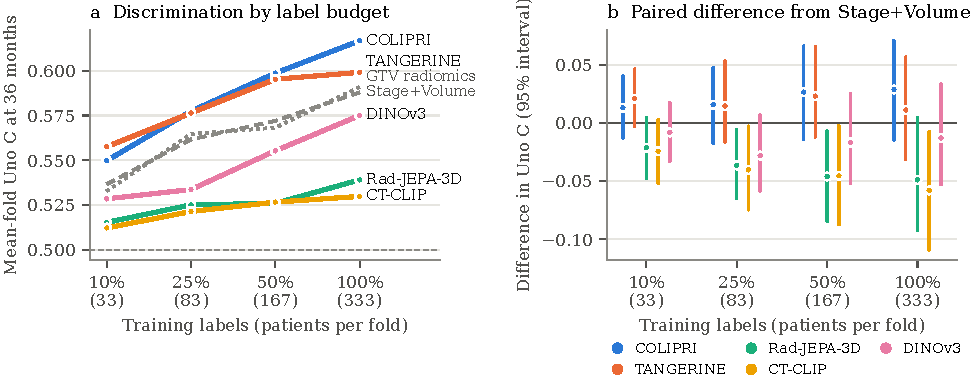
\includegraphics[width=\linewidth]{figures/results_rq2.pdf}
\caption{RQ2: discrimination by training-label budget. (a) Mean-fold Uno C of the frozen PCA16 heads and of the \model{Stage+Volume} (dashed) and radiomic (dotted) baselines, refitted on nested subsets of each development set (ten draws below 100\%) and evaluated on the unchanged test folds. (b) Paired difference of each encoder from \model{Stage+Volume} at each budget, with 95\% intervals (300 resamples). None was significant after Holm correction.}
\label{fig:rq2}
\end{figure}


\subsection{RQ3: How sensitive are the representations and their survival predictions to the tumour?}\label{sec:res-rq3}

The four tumour analyses, described in Section~\ref{sec:perturbation} (Figure~\ref{fig:rq3design}), are summarized in Figure~\ref{fig:rq3}.

\begin{figure}[!t]
\centering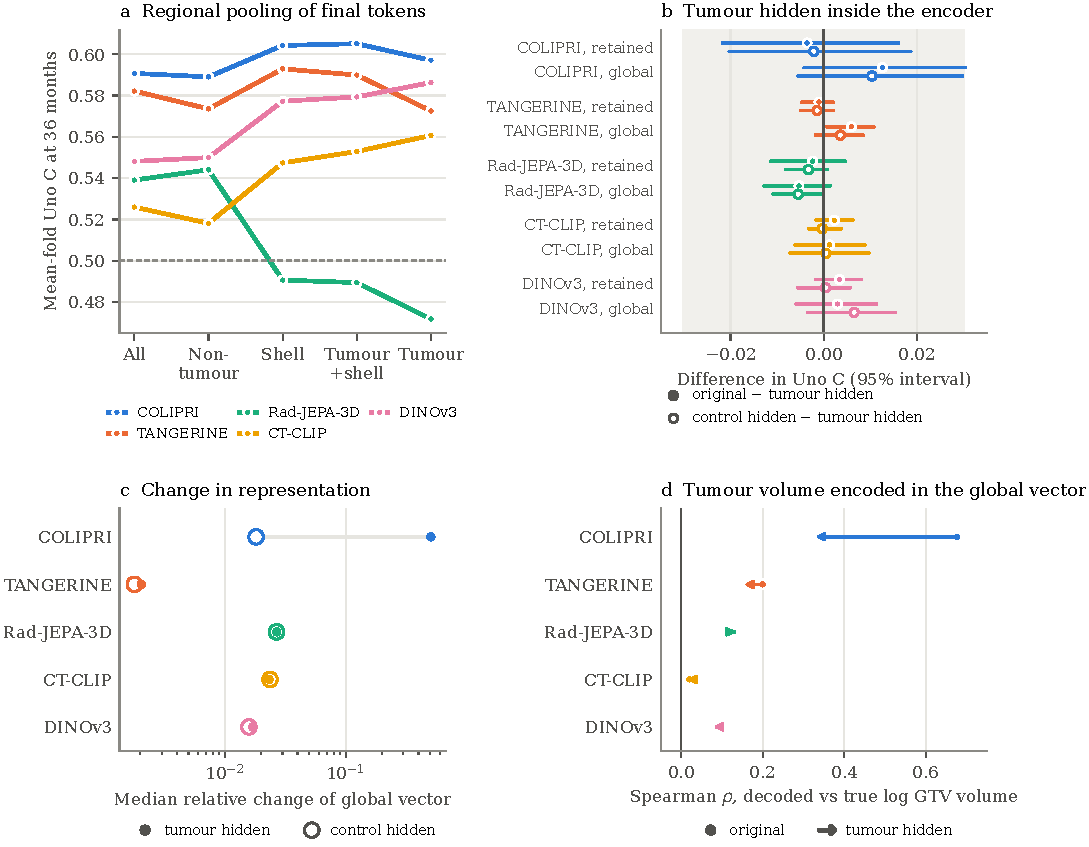
\includegraphics[width=\linewidth]{figures/results_rq3.pdf}
\caption{RQ3: dependence on the tumour. (a) Mean-fold Uno C of the frozen head applied to final tokens pooled over regions defined by the GTV (Section~\ref{sec:perturbation}); the all-token pool is a uniform mean and differs from the encoders' global vectors. (b) Native-token masking in the 403 patients with a matched control: paired differences in Uno C, with retained (mean of tokens visible in every condition) and global vectors; shaded area, $\pm0.03$. Intervals use 300 paired resamples and are not adjusted for multiplicity. (c) Median relative change of the global vector when the tumour or the matched control was hidden (logarithmic scale). (d) Decodability of log GTV volume from the global vector (PCA16 ridge probe), original and with the tumour hidden.}
\label{fig:rq3}
\end{figure}

\paragraph{Regional pooling.} Pooling the final tokens over different regions changed discrimination little except for Rad-JEPA-3D (Figure~\ref{fig:rq3}a). For every encoder, the non-tumour pool was within 0.009 of the all-token pool, because the tumour occupies few token positions. For COLIPRI, the tumour pool differed from the all-token pool by $+0.006$ ($-0.019$ to $+0.031$), and the shell and tumour-plus-shell pools scored highest (0.604 and 0.605). Restricting Rad-JEPA-3D to tumour tokens lowered its discrimination to 0.472, $-0.067$ ($-0.110$ to $-0.025$) relative to all tokens. CT-CLIP and DINOv3 improved numerically with tumour pooling, by $+0.035$ ($-0.015$ to $+0.081$) and $+0.038$ ($-0.005$ to $+0.075$). For TANGERINE and Rad-JEPA-3D, adding the shell to the tumour raised discrimination by about 0.02 (lower bounds $+0.001$ and $+0.004$).

\paragraph{Native-token masking.} Hiding the tumour inside the encoder barely changed discrimination (Figure~\ref{fig:rq3}b). In the 403 patients with a valid control, the original-minus-masked difference on the retained tokens, the primary pooling, ranged from $-0.004$ (COLIPRI; $-0.022$ to $+0.016$) to $+0.003$ (DINOv3), and every interval lay within the equivalence margin. With the global vector, the largest differences were $+0.013$ for COLIPRI ($-0.004$ to $+0.030$), $+0.006$ for TANGERINE ($+0.001$ to $+0.011$) and $-0.005$ for Rad-JEPA-3D ($-0.013$ to $+0.001$). The differences between the control-hidden and tumour-hidden conditions were of the same size, so hiding the tumour was no more harmful than hiding any comparable region.

The representations themselves responded differently (Figure~\ref{fig:rq3}c). Hiding the tumour changed the COLIPRI global vector by a median of 51\%, against 2\% for the matched control. For the other four encoders, the tumour and the control changed the global vector by the same amount (0.2\% to 2.7\%), so these vectors were insensitive to the tumour specifically.

\paragraph{Fixed head.} When the head fitted on original embeddings was applied unchanged to the masked ones, COLIPRI fell from 0.623 to 0.610 with the global vector (difference $+0.013$; $-0.002$ to $+0.029$), with a similar difference for the retained tokens ($+0.012$; $-0.003$ to $+0.028$), whereas hiding the control changed it by less than 0.001. The rank correlation between original and masked risk scores was 0.92 for COLIPRI and at least 0.996 for every other encoder. The fitted COLIPRI model therefore used some tumour-derived information, but losing it cost little discrimination.

\paragraph{Clinical-variable probing.} The embeddings explain why (Figure~\ref{fig:rq3}d). The COLIPRI global vector encoded tumour volume (Spearman $\rho=0.68$) and T3--T4 category (AUC 0.70); hiding the tumour reduced these to 0.32 (difference 0.36; 0.28 to 0.44) and 0.55 (difference 0.15; 0.09 to 0.19). Age ($\rho=0.70$ to 0.69) and stage III (AUC 0.70 to 0.72) were unaffected. The other encoders encoded tumour volume weakly ($\rho\leq0.20$) but encoded sex strongly (AUC 0.78 to 0.999); TANGERINE also encoded age ($\rho=0.71$) and stage III (AUC 0.75), all unchanged by masking. Histology was not decodable (AUC 0.42--0.64).

Only COLIPRI was sensitive to the tumour, and it encoded tumour size, the block that added most to the clinical covariates in RQ1. Yet hiding the tumour halved the decodable volume and lowered discrimination by at most 0.013, indicating that most of the prognostic information in these representations was carried by the rest of the scan.


\subsection{RQ4: Do discrimination, incremental clinical value and calibration transfer to an external cohort?}\label{sec:res-rq4}

\begin{table}[!htbp]
\centering\footnotesize
\caption{External evaluation in NSCLC-Radiogenomics (143 patients, 33 deaths by 36 months). Models were fitted on all 416 LUNG1 patients and frozen before external outcomes were read. Internal and external values are Uno C at 36 months; internal is the mean-fold LUNG1 estimate. External intervals come from 2,000 patient resamples and condition on the frozen models. $p_\mathrm{Holm}$ tests external Uno C against 0.5, Holm-adjusted across all models. Calibration slope: coefficient of the linear predictor in an external Cox regression (1 is ideal). Predicted: mean predicted 36-month mortality with the LUNG1 baseline hazard; observed Kaplan--Meier mortality was 0.25. The Hosny zero-shot score has no baseline hazard. $^{\ddagger}$Exploratory: fixed LoRA configuration, trained on all LUNG1 patients after the external cohort had been examined; it was chosen on the COLIPRI and TANGERINE test folds. Internal values are the LoRA estimates of Table~\ref{tab:trainable_results}. $^{\dagger}$Unadjusted $p$ against 0.5; the exploratory LoRA analysis was not corrected for multiplicity. $^{\S}$Training did not converge; predicted risks were almost constant.}
\label{tab:external}
\begin{tabular}{@{}lrlrrr@{}}
\toprule
Model & Internal & External (95\% interval) & $p_\mathrm{Holm}$ & Slope & Predicted \\
\midrule
\multicolumn{6}{@{}l}{\textit{Clinical and radiomic}}\\
\model{Clinical} & 0.529 & 0.595 (0.493 to 0.698) & 0.402 & 1.73 & 0.66 \\
\model{Clinical+Volume} & 0.565 & 0.646 (0.547 to 0.749) & 0.067 & 1.76 & 0.63 \\
\model{Stage+Volume} & 0.588 & 0.605 (0.508 to 0.702) & 0.367 & 3.24 & 0.67 \\
GTV radiomics & 0.591 & 0.617 (0.508 to 0.723) & 0.299 & 0.45 & 0.62 \\
\multicolumn{6}{@{}l}{\textit{Clinical and image}}\\
\model{Clinical+Volume+COLIPRI} & 0.599 & 0.653 (0.557 to 0.748) & 0.027 & 1.84 & 0.64 \\
\model{Clinical+Volume+Radiomics+COLIPRI} & 0.606 & 0.652 (0.555 to 0.751) & 0.040 & 0.92 & 0.67 \\
\multicolumn{6}{@{}l}{\textit{Frozen image representations}}\\
COLIPRI & 0.617 & 0.627 (0.540 to 0.719) & 0.077 & 1.90 & 0.65 \\
TANGERINE & 0.599 & 0.649 (0.550 to 0.741) & 0.041 & 0.62 & 0.50 \\
Rad-JEPA-3D & 0.539 & 0.530 (0.436 to 0.627) & 1.000 & 0.05 & 0.84 \\
CT-CLIP & 0.530 & 0.482 (0.388 to 0.581) & 1.000 & -0.57 & 0.64 \\
DINOv3 & 0.575 & 0.643 (0.556 to 0.730) & 0.021 & 1.26 & 0.85 \\
Pai lesion encoder & 0.555 & 0.547 (0.446 to 0.646) & 1.000 & 0.48 & 0.66 \\
Hosny zero-shot & 0.566 & 0.540 (0.432 to 0.643) & 1.000 & 0.13 & -- \\
\multicolumn{6}{@{}l}{\textit{Exploratory LoRA adaptation}$^{\ddagger}$}\\
COLIPRI, LoRA & 0.639 & 0.687 (0.606 to 0.768) & $<$0.001$^{\dagger}$ & 0.79 & 0.53 \\
TANGERINE, LoRA & 0.630 & 0.633 (0.536 to 0.728) & 0.007$^{\dagger}$ & 0.57 & 0.61 \\
Rad-JEPA-3D, LoRA & 0.520 & 0.442 (0.329 to 0.556) & 0.311$^{\dagger}$ & -0.28 & 0.81 \\
CT-CLIP, LoRA$^{\S}$ & 0.500 & 0.505 (0.405 to 0.606) & 0.924$^{\dagger}$ & 5.52 & 0.68 \\
DINOv3, LoRA & 0.577 & 0.623 (0.528 to 0.721) & 0.012$^{\dagger}$ & 0.22 & 0.48 \\
\bottomrule
\end{tabular}
\end{table}

Externally, discrimination was maintained or higher for COLIPRI, TANGERINE and DINOv3 and lost for Rad-JEPA-3D, CT-CLIP and the tumour-centred deep models (Table~\ref{tab:external}; Figure~\ref{fig:rq4}a). TANGERINE reached 0.649 (0.550 to 0.741), DINOv3 0.643 and COLIPRI 0.627, compared with 0.646 for \model{Clinical+Volume} and 0.605 for \model{Stage+Volume}. After Holm correction, TANGERINE ($p_\mathrm{Holm}=0.041$) and DINOv3 (0.021) exceeded chance, as did \model{Clinical+Volume+COLIPRI}, \model{Clinical+Volume+DINOv3} and both \model{Clinical+Volume+Radiomics+Image} models, whereas COLIPRI (0.077), \model{Clinical+Volume} (0.067) and \model{Stage+Volume} (0.37) did not. Rad-JEPA-3D (0.530), CT-CLIP (0.482), the Pai lesion encoder (0.547) and Hosny zero-shot (0.540) were at chance. The ranking of the 22 models was largely preserved (Spearman $\rho=0.67$, $p<0.001$).

None of the four primary contrasts was significant or equivalent. COLIPRI exceeded \model{Stage+Volume} by 0.021 ($-0.068$ to $0.126$), the Pai lesion encoder by 0.080 ($-0.031$ to $0.195$) and Hosny zero-shot by 0.087 ($-0.046$ to $0.231$), and \model{Clinical+Volume+COLIPRI} exceeded \model{Clinical+Volume} by 0.007 ($-0.052$ to $0.071$); all $p_\mathrm{Holm}\geq0.67$. The minimum detectable differences were 0.088 for the clinical increment and 0.13 to 0.20 for the others, several times the size of the internal differences, so these contrasts are uninformative.

Absolute risks did not transport (Figure~\ref{fig:rq4}b). Observed 36-month mortality was 25\%, whereas mean predicted mortality ranged from 37\% to 85\% and was at least 58\% for every model except TANGERINE (50\%) and \model{Clinical+Volume+TANGERINE} (37\%). Calibration slopes ranged from $-0.57$ (CT-CLIP) to 3.24 (\model{Stage+Volume}); for COLIPRI it was 1.90, indicating that its predicted risks were not spread widely enough for the external population.

In the exploratory external LoRA analysis, adaptation improved external discrimination only for COLIPRI, which reached 0.687 (0.606 to 0.768), 0.060 above its frozen head (0.004 to 0.120). For the other encoders, LoRA was at or below the frozen head: TANGERINE $-0.016$ ($-0.107$ to $+0.073$), DINOv3 $-0.019$ ($-0.101$ to $+0.067$) and Rad-JEPA-3D $-0.088$ ($-0.172$ to $-0.011$), with Rad-JEPA-3D falling below chance (0.442). As internally, CT-CLIP did not train and its predicted risks were almost constant. Intervals are not adjusted for multiplicity, and the COLIPRI and TANGERINE models were trained in FP16 rather than BF16. Because the configuration was chosen on LUNG1 test folds and the analysis was added after the external cohort had been examined, the single COLIPRI gain is a hypothesis for independent testing, not evidence that adaptation transfers.

Risk ordering by the stronger frozen encoders therefore transported to a population with a different stage, treatment and scanner mix, whereas their incremental value over clinical models could not be resolved with 33 external events, and their absolute risks required recalibration.

\begin{figure}[!htbp]
\centering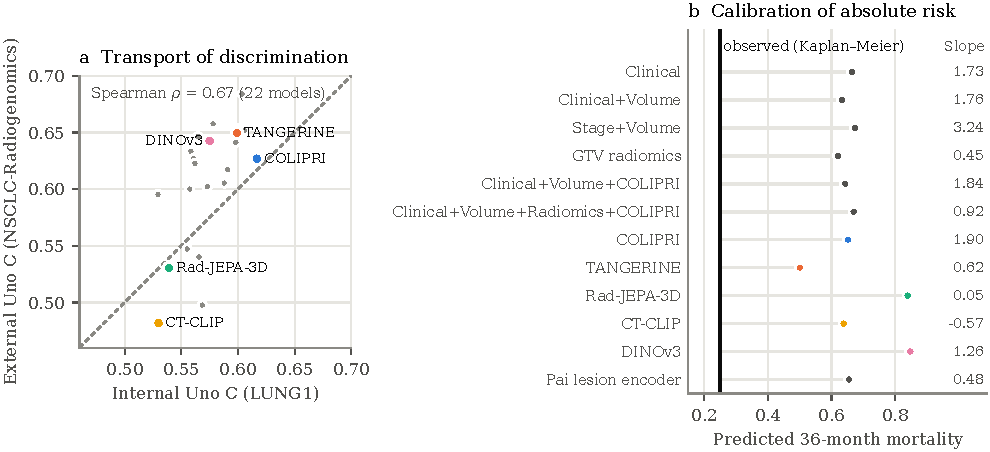
\includegraphics[width=\linewidth]{figures/results_rq4.pdf}
\caption{RQ4: external evaluation in NSCLC-Radiogenomics (143 patients). (a) Internal (LUNG1 mean-fold) against external Uno C at 36 months for the 22 frozen models; coloured points are the frozen encoders, grey points the clinical, radiomic, tumour-centred and combined models; the dashed line is identity. (b) Mean predicted 36-month mortality with the LUNG1 baseline hazard against the observed Kaplan--Meier mortality (vertical line); the column on the right gives the external calibration slope.}
\label{fig:rq4}
\end{figure}
